% !TEX root = ./rosbook_jp.tex
%-------------------------------------------------------------------------------
\chapterimage{chapter_head_3.pdf}

%-------------------------------------------------------------------------------
\chapter{ROSの基本知識}\index{ROSの基本知識}

%-------------------------------------------------------------------------------
\section{ROSで使われる専門用語}\index{ROSで使われる専門用語}

ROSでは多くの独特の概念や用語が使われる。本節では、頻繁に使用されるROSの用語についてまとめて解説する。ただし、ここですべて理解する必要はなく、わからない用語が出てきても、先に読み進めていただきたい。これらの用語は、実際にROSを利用していけば、自然と身につくものである。

%-------------------------------------------------------------------------------
\subsubsection{マスター(master)}
マスター(master)は、ノード間の接続とメッセージ通信の実現に必要なサーバ(ネームサーバ)である。マスターの起動にはroscoreコマンドを用いる。マスターが起動すると、マスターは各ノードの名前を登録し、ノードとの間で必要な情報を送受信する。マスターが起動していなければ、ノード間の接続やメッセージ通信を行うことができない。
マスターは、HTTPベースのプロトコルであるXMLRPCを使用してノードと通信する。XMLRPCでは、マスターとノードは常に接続を維持する必要はなく、ノードは必要な場合にのみマスターに接続して、ノード自身の情報や他のノードの情報をやり取りする。ROSの ノード間通信は、お互いの接続状態を監視していないため、大規模なシステムでも利用できる。また、XMLRPCは計算負荷が小さく、さらに様々なプログラミング言語をサポートしている。

%-------------------------------------------------------------------------------
\subsubsection{ノード(node)}
ノード(node)は、ROSの最小の構成要素であり、個々の実行プログラムである。ノードは個別の処理毎に作成され、多くのシステムで繰り返し利用できるように設計される。例えば移動ロボットの場合、センサドライバ、センサデータ処理、障害物検出、モータ駆動、エンコーダ入力、ナビゲーションなど、動作に必要な処理を細分化し、それぞれの処理を実装したノードを組み合わせてシステムを構築する。
ノードを実行する際には、配信者(publisher)、購読者(subscriber)、トピック、サービス名、メッセージの形式、URIアドレスとポートをマスターに登録する。これらの情報を基に、各ノードは、ノード間でトピックメッセージ通信とサービスメッセージ津伸を利用して情報を送受信する。
ノードとマスター間の通信にはXMLRPCを利用する。また、ノード同士の通信方式には2種類あり、接続要請と接続応答にはXMLRPCを、メッセージ通信には2点間通信方式であるTCP/IP通信を改良したTCPROSを使用する。すなわち、ノード間の通信はマスターを介して行うわけではない。ノードのURIアドレスには、ノードを実行しているPCのROS\_HOSTNAME変数を使用し、ポートは任意の値に設定される。

%-------------------------------------------------------------------------------
\subsubsection{パッケージ(package)}
ROSのアプリケーションはパッケージ(package)単位で開発される。ROS Indigoは2015年5月20日現在、約1,660個(http://www.ros.org/debbuild/indigo.html)のパッケージを提供しており、また、ユーザーが開発し公開したパッケージは約5,400個(http://rosindex.github.io/stats/)にもなる。

%-------------------------------------------------------------------------------
\subsubsection{メタパッケージ(metapackage)}
メタパッケージ(metapackage)は、共通の目的を持ったパッケージを集めたパッケージのセットである。

%-------------------------------------------------------------------------------
\subsubsection{メッセージ(Message)}
メッセージ(message、msg)とは、ノード間でやり取りされる情報である。メッセージは整数型、浮動小数点型、論理型などの変数で構成されている。また、この他にもユーザーが自由にメッセージの型を設定でき、例えば配列型やネスト構造(他のファイルで宣言されたメッセージ型を内包したメッセージ型)なども使用できる。メッセージを利用した通信方法には、一方向のメッセージ送受信方式であるトピック(topic)メッセージ通信と、双方向のメッセージ送受信方式であるサービス(service)メッセージ通信がある。

%-------------------------------------------------------------------------------
\subsubsection{トピック(Topic)}
トピック(topic)は一方向で非同期方式のメッセージ送受信方式である。配信者(publisher)が配信したいデータをもつとき、そのデータを変数として含むメッセージに固有のトピック名を付けてマスターに登録する。その後、このトピックの受信を希望する購読者(subscriber)は、登録されたトピック名に対応する配信者の情報をマスターから受け取る。この情報に基づいて,購読者は配信者と直接接続して、メッセージをトピックで送受信する。

%-------------------------------------------------------------------------------
\subsubsection{配信および配信者(publish and publisher)}
配信(publish)とは、各トピックで定義されたメッセージを送信することをいう。配信者(publisher)は、メッセージを配信するために、トピック名などの情報をマスターに登録する。トピックを購読したい購読者は、マスターから必要な情報を得て配信者と接続し、メッセージを受け取る。一つのノードは複数の配信者を利用できる。以降では、配信者を実行するノードを「配信者ノード」と呼ぶ。

%-------------------------------------------------------------------------------
\subsubsection{購読および購読者(subscribe and subscriber)}
購読(subscribe)とは、各トピックで定義されたメッセージを受信することをいう。購読者(subscriber)は、トピック名などの情報をマスターに登録し、購読しようとするトピックの配信者の情報をマスターから受ける。この情報に基づいて購読者は、配信者と直接接続してメッセージを受け取る。一つのノードで複数の購読者を利用できる。以降では、購読者を実行するノードを「購読者ノード」と呼ぶ。

%-------------------------------------------------------------------------------
\subsubsection{サービス(service)}
サービス(service)とは、メッセージ同期方式の通信方式である。上述した配信と購読に基づくトピックメッセージ通信方式は非同期方式であり、データの送受信を効率的に行うことができる。また、一度接続処理を行えば、その後は連続的にメッセージを送受信できるので、継続してメッセージを送信しなければならないセンサデータの通信処理に適している。しかし、場合によっては、リクエスト(request)とレスポンス(response)によって構成される、同期方式のメッセージ交換方式も必要となる。ROSは、これをサービスメッセージ通信と呼ぶ通信方式で提供する。サービスメッセージ通信は、リクエストを受け取ると情報を送信するサービスサーバ(service server)と、リクエストを送信し情報を受け取るサービスクライアント(service client)から構成される。サービスは、トピックとは異なり、一回限りのメッセージ通信である。サービスのリクエストとレスポンスが完了すると、二つのノードの接続は一度切断される。

%-------------------------------------------------------------------------------
\subsubsection{サービスサーバ(service server)}
サービスサーバ(service server)は、リクエストを入力として受け取り、レスポンスを出力するサービスメッセージ通信のサーバである。リクエストとレスポンスはメッセージであり、サービスサーバはリクエストを受信すると、指定されたサービスを実行し、その結果をサービスクライアントに送信する。通常、サービスサーバは、決められた命令を受けて、特定の処理を実行するノードで使用される。

%-------------------------------------------------------------------------------
\subsubsection{サービスクライアント(service client)}
サービスクライアント(service client)は、リクエストを出力し、レスポンスを受け取るサービスメッセージ通信のクライアントである。リクエストとレスポンスはメッセージであり、サービスクライアントはリクエストをサービスサーバに送信し、そのレスポンスを受信する。サービスクライアントは、ある定められたコマンドをサービスサーバへ送信し、結果を受けるノードで使用される。

%-------------------------------------------------------------------------------
\subsubsection{catkinビルドシステム(catkin build system)}
catkin(キャッキン)はROSのビルドシステムである。catkinビルドシステムは、一般的なビルドシステムであるCMake(Cross Platform Make)を拡張したものであり、CMakeと同様に、パッケージのフォルダ内のCMakeLists.txtファイルにビルド環境を記述している。catkinはROS Fuerteバージョンからアルファテストを開始して、Groovyでコアパッケージがcatkinビルドシステムに切り代わり、Hydroバージョン以降は全システムで使えるようになった。catkinビルドシステムを用いると、パッケージのビルド、パッケージ管理、依存関係パッケージの自動インストールなどが容易に行える。

%-------------------------------------------------------------------------------
\subsubsection{ROSビルドシステム(rosbuild system)}
ROSビルド(rosbuild)はcatkinビルドシステム以前に使用されたビルドシステムであり、今も一部のユーザーが使用している。しかしROSのバージョンの互換性のために残されたものであり、今後は使用されないため、本書ではrosbuildの使用は推奨しない。もし、rosbuildビルドシステムを使用した以前のパッケージを使用する必要がある場合、catkinビルドシステムへの修正を試みるべきである。

%-------------------------------------------------------------------------------
\subsubsection{roscore}
roscoreはROSマスターを実行するためのコマンドである。同じネットワークセグメントであれば、どのPCで実行してもよい。ただし、マルチROSマスターをサポートしている場合を除いては、roscoreは同じネットワーク内で1つのみ実行できる。ノードを起動する際には、ネットワーク内の1台のPCで必ずマスターを起動しておく必要がある。またユーザーは、ノードを実行するネットワーク内のすべてのPCで、マスターが実行されているPCのURIやIPアドレス、ポート番号を、「~/.bashrc」ファイルのROS\_MASTER\_URI変数に設定しておかなければならない。ROS\_MASTER\_URI変数が設定されていない場合は、ノードを実行したPCのIPアドレスと11311ポートが使用される。

%-------------------------------------------------------------------------------
\subsubsection{パラメータ(parameter)}
パラメータ(parameter)とは、ノード内で使用され、ノード実行中に変更可能な変数である。パラメータは規定値が設定されており、ノード実行中に外部からの読み取り、または書き込みができる。例えば、外部デバイスを接続したUSBポートの番号やカメラキャリブレーション値、モータの速度やコマンドの最大値と最小値などをノード実行中に外部から確認することや、値を変更することができる。

%-------------------------------------------------------------------------------
\subsubsection{パラメータサーバ(parameter server)}
パラメータサーバ(parameter server)とは、ノードでパラメータを使用する際、パラメータの書き込みや読み込みを行うサーバである。パラメータサーバは、マスターの起動と同時に自動的に立ち上がる。エンコード形式にはXMLを採用し、伝送方式にはリクエスト/レスポンス方式のHTTPプロトコルであるXMLRPCを使用する。

%-------------------------------------------------------------------------------
\subsubsection{rosrun}
rosrunはROSにおける最も基本的な実行コマンドである。パッケージ内の1つのノードを実行する際に使用する。

%-------------------------------------------------------------------------------
\subsubsection{roslaunch}
rosrunが1つのノードを実行するコマンドであるのに対し、roslaunchは複数のノードを実行するコマンドである。さらにパッケージのパラメータやノード名の変更、ノードのNamespaceの設定、ROS\_ROOTとROS\_PACKAGE\_PATHの設定、環境変数の変更など、多くのオプションを備えたROSコマンドである。roslaunchは「.launch」という拡張子のファイルを使用して、実行ノードの設定ができる。roslaunchの形式はXMLに基づいており、XMLタグ形式でオプションを設定する。

%-------------------------------------------------------------------------------
\subsubsection{bag}
ROSで送受信されるメッセージのデータをファイルとして保存する際の形式がbagである。「.bag」という拡張子を使う。ROSは、bagとして保存したメッセージを後に必要に応じて再生することで、実行時の状況をそのまま再現できる。たとえば、センサーを利用したロボットの走行実験を行うとき、bagを使用してセンサーのデータをメッセージの形式で保存する。その後、保存しておいたbagファイルを再生することで、実際にロボットを走行させなくても、実験時のセンサーの値を繰り返し使用できる。このbagの記録・再生の機能を活用すれば、プログラムの修正が多い複雑なアルゴリズムの開発を効率化できる。

%-------------------------------------------------------------------------------
\subsubsection{ROS Wiki}
ROSの各パッケージと機能を説明するページ(http://wiki.ros.org/)である。このページには各パッケージの簡単な説明、使用されるパラメータ、著作者、ライセンス、ホームページ、リポジトリ、チュートリアルなどが記載されている。

%-------------------------------------------------------------------------------
\subsubsection{リポジトリ(repository)}
リポジトリ(repository)は、パッケージが格納されているウェブ上のURLアドレスで、svn、hg、gitなどのソース管理システムを利用して、障害情報、開発記録、ソースコードのダウンロードなどを管理している。公開されたパッケージでは、各パッケージのWikiにリポジトリを記載している。

%-------------------------------------------------------------------------------
\subsubsection{rqtグラフ(rqt\_graph)}
rqt\_graph(rqt\_graph)は、ノード、トピック、配信者、購読者の関係を視覚的にわかりやすく表示するツールである。実行コマンドはrqt\_graph、あるいはrosrun rqt\_graph rqt\_graphであり、両者に違いはない。なお、これらは実行中のトピックメッセージ通信をグラフ形式で表示するものであり、通信が一度しか行われないサービスメッセージ通信は表示できない。

%-------------------------------------------------------------------------------
\subsubsection{名前(name)}
ノード、パラメータ、トピック、サービスには、すべて固有の名前(name)が付けられている。各ノードでパラメータ、トピック、サービスを利用するときには、マスターに登録された名前に基づいて、他のノードの検索、接続、メッセージ送受信を行う。また、名前は起動時に変更でき、同じノード、パラメータ、トピック、サービスであっても別の名前で登録すれば重複して使用できるなど、極めて柔軟である。

%-------------------------------------------------------------------------------
\subsubsection{クライアントライブラリ(client library)}
ROSは、特定のプログラミング言語にできるだけ依存しないように、クライアントライブラリ(client library)として、各種の言語による開発環境を提供している。主な言語には、C ++、Python、Lispなどがあり、さらにjava、lua、.NET、EusLisp、Rなどの言語も使用できる。クライアントライブラリは、これまでroscpp、rospy、roslisp、rosjava、roslua、roscs、roseus、PhaROS、rosRなどが開発されている。

%-------------------------------------------------------------------------------
\subsubsection{TCPROS}
メッセージとサービスで使用されるTCP/IPベースのメッセージ伝送方式である。

%-------------------------------------------------------------------------------
\subsubsection{UDPROS}
メッセージとサービスで使用されるUDPベースのメッセージ伝送方式である。あまり使用されない。

%-------------------------------------------------------------------------------
\subsubsection{CMakeLists.txt}
ROSのビルドシステムであるcatkinはCMakeを拡張したものである。パッケージフォルダ内のCMakeLists.txtファイルにビルド環境を記述している。

%-------------------------------------------------------------------------------
\subsubsection{package.xml}
パッケージの情報を記載したXMLファイルである。パッケージの名前、著作者、ライセンス、依存性パッケージなどが記載されている。

%-------------------------------------------------------------------------------
\section{メッセージ通信}\index{メッセージ通信}

本節では、ROSの重要な機能であるノード間のメッセージ通信注1,2について説明する。作業目的に応じて細分化されたノードは、他のノードと処理結果を送受信(メッセージ通信)することで一つの大きなプログラムになる。ノード間のメッセージ通信には、トピックメッセージ通信とサービスメッセージ通信の2つの方法がある。これらの通信方法について、以下で詳しく見ていこう。

%-------------------------------------------------------------------------------
\subsection{トピックメッセージ通信}
トピックメッセージ通信は、図3-1のように、情報を送信する配信者と情報を受信する購読者が、トピックと呼ばれる形式でメッセージを送受信するものである。一つの配信者から複数の購読者への通信や、逆に複数の配信者から一つの購読者への通信も可能である。もちろん、一つの配信者から一つの購読者や、多数の配信者から多数の購読者への通信も可能である。トピックメッセージ通信は、例えば移動ロボットの両輪のエンコーダ値を計測して、ロボットの現在位置であるオドメトリ(odometry)情報を計算し、得られた位置情報をトピックメッセージ(x、y、θ)として送信する場合など、一方向で連続的なメッセージの送受信に用いられる。

\begin{figure}[htp]
  \centering
  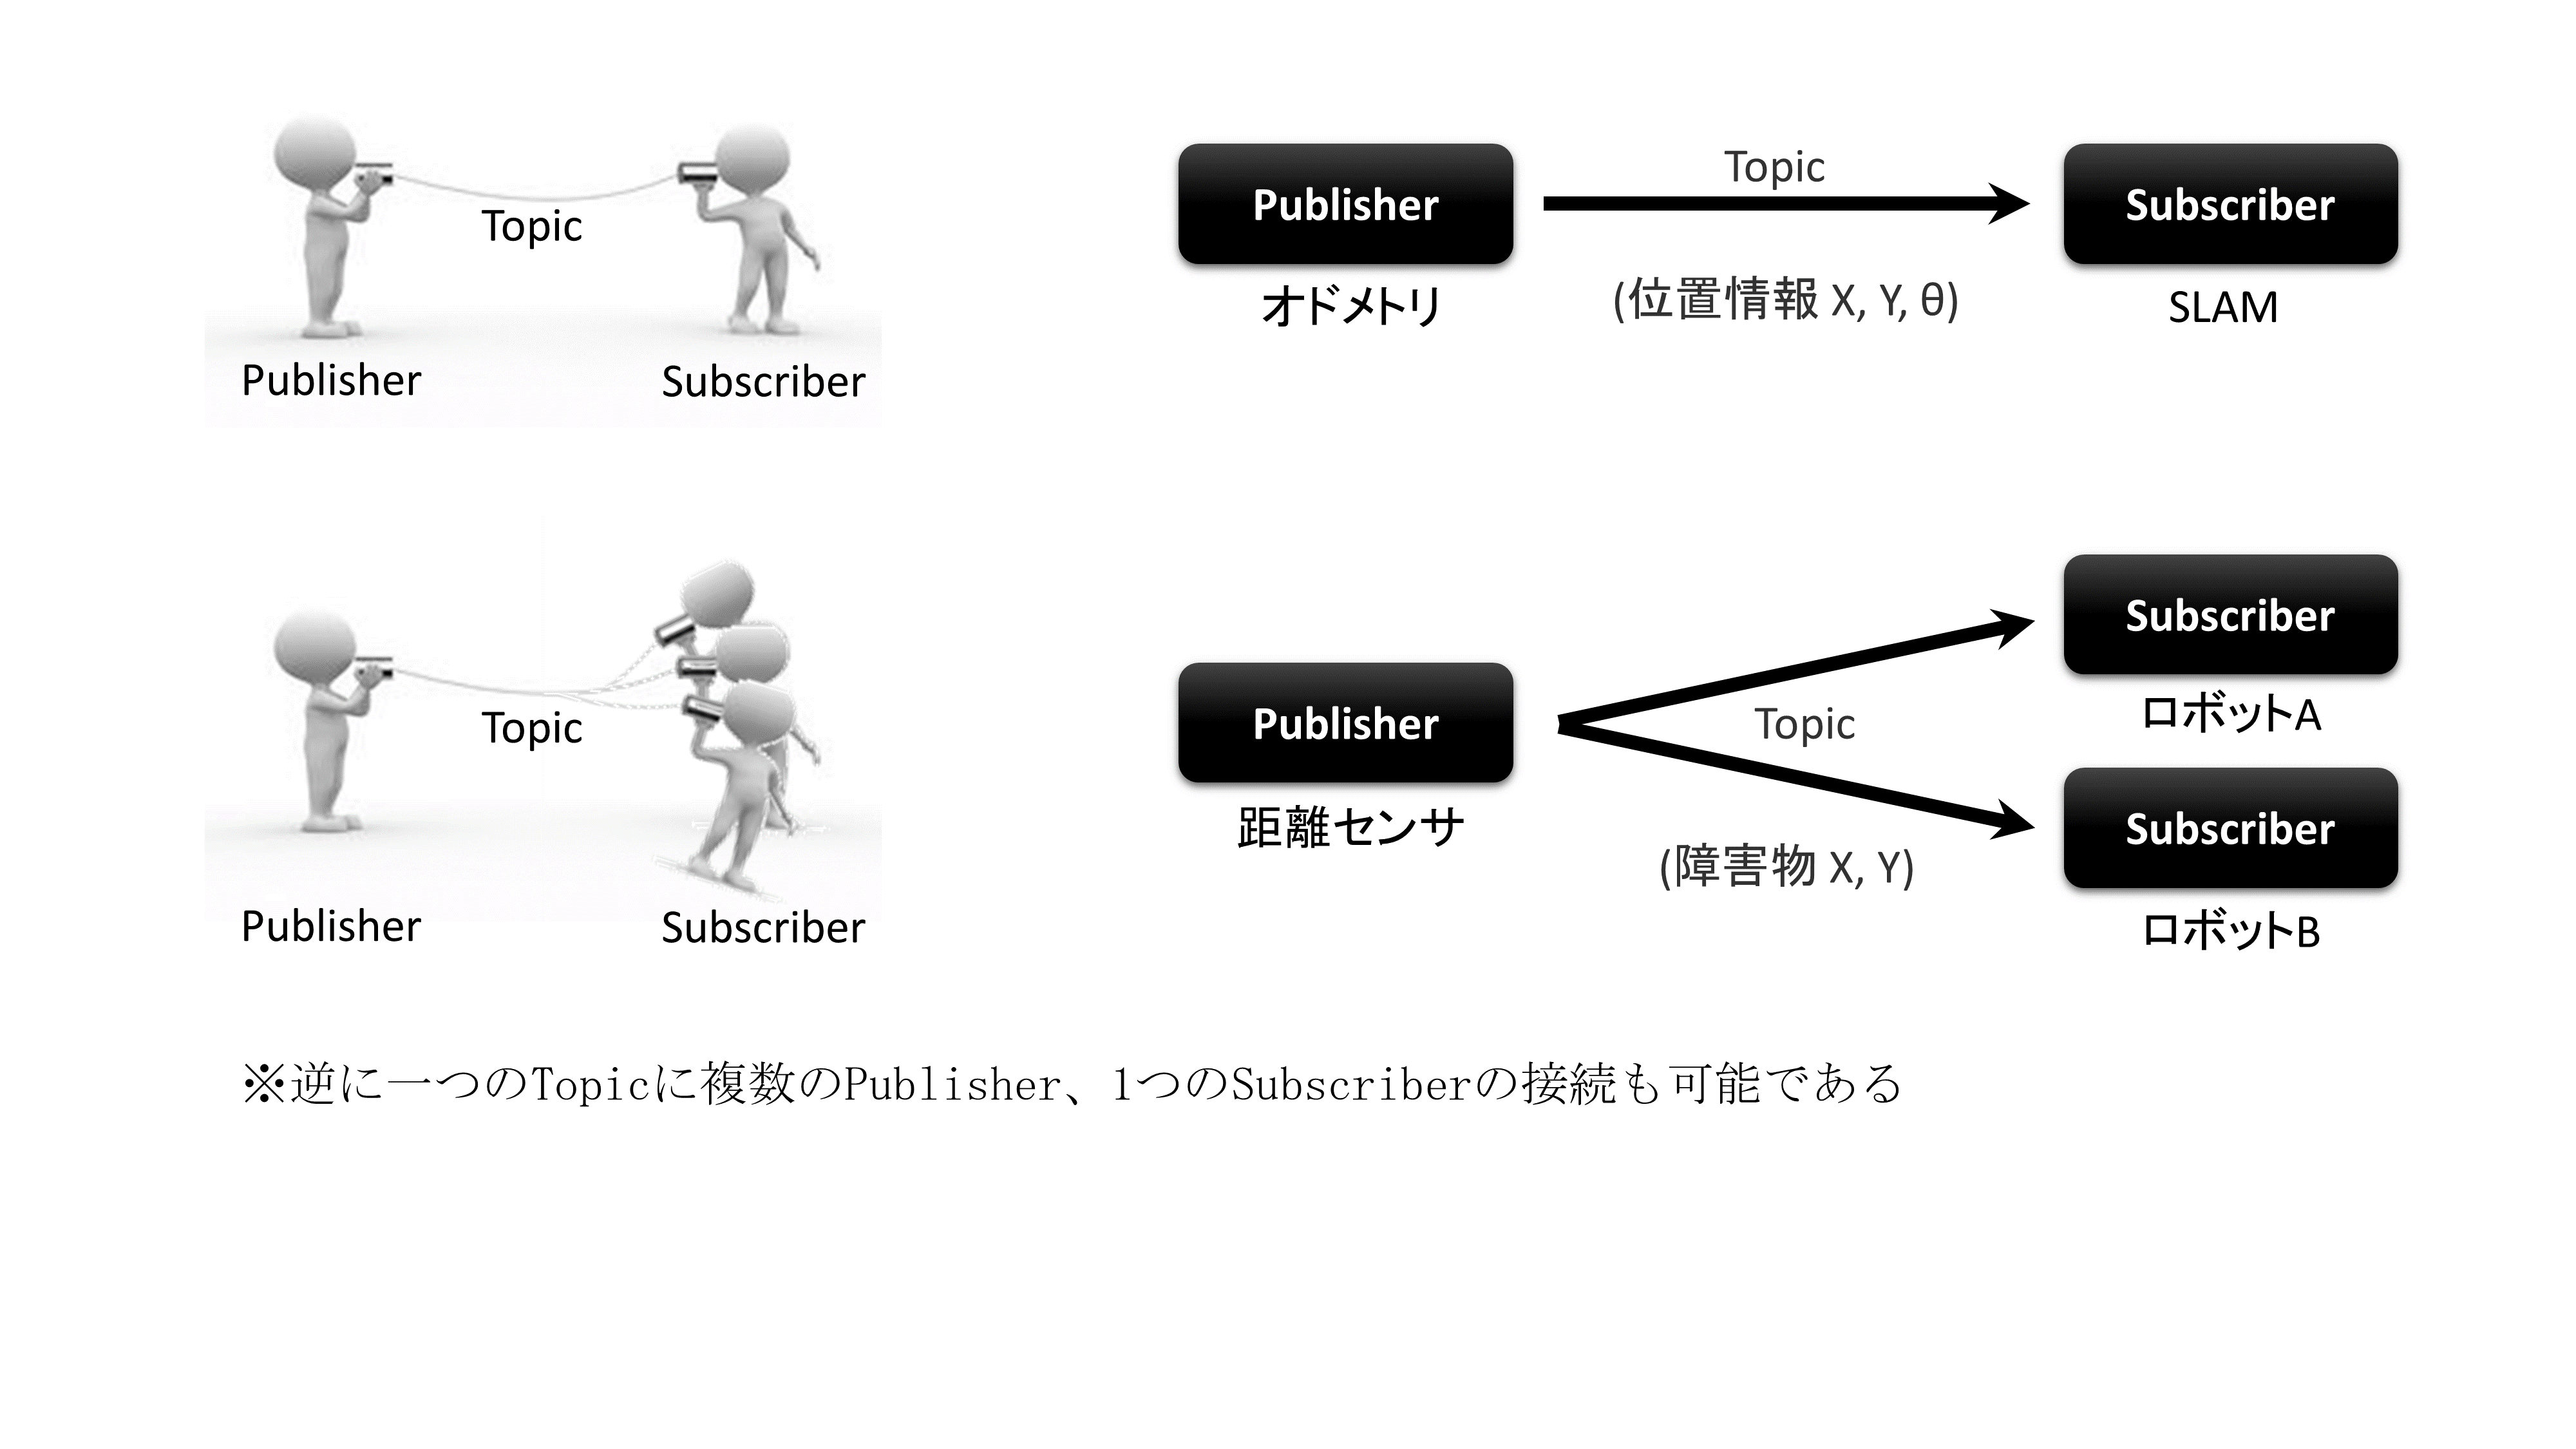
\includegraphics[width=\columnwidth]{pictures/chapter3/pic_03_01.png}
  \caption{トピックメッセージ通信}
\end{figure}

%-------------------------------------------------------------------------------
\subsection{サービスメッセージ通信}
サービスメッセージ通信とは、図3-2に示すようにサービスをリクエスト(request)するサービスクライアント(service client)と、レスポンス(response)を返すサービスサーバ(service server)間の、双方向サービスメッセージ通信である。例えば、図3-2に示すように、クライアントがサーバに現在時刻をリクエストすると、サーバは時間を調べてクライアントにレスポンスを返す。このサービスメッセージ通信は、トピックメッセージ通信とは異なり、一対一の通信のみが可能である。

\begin{figure}[htp]
  \centering
  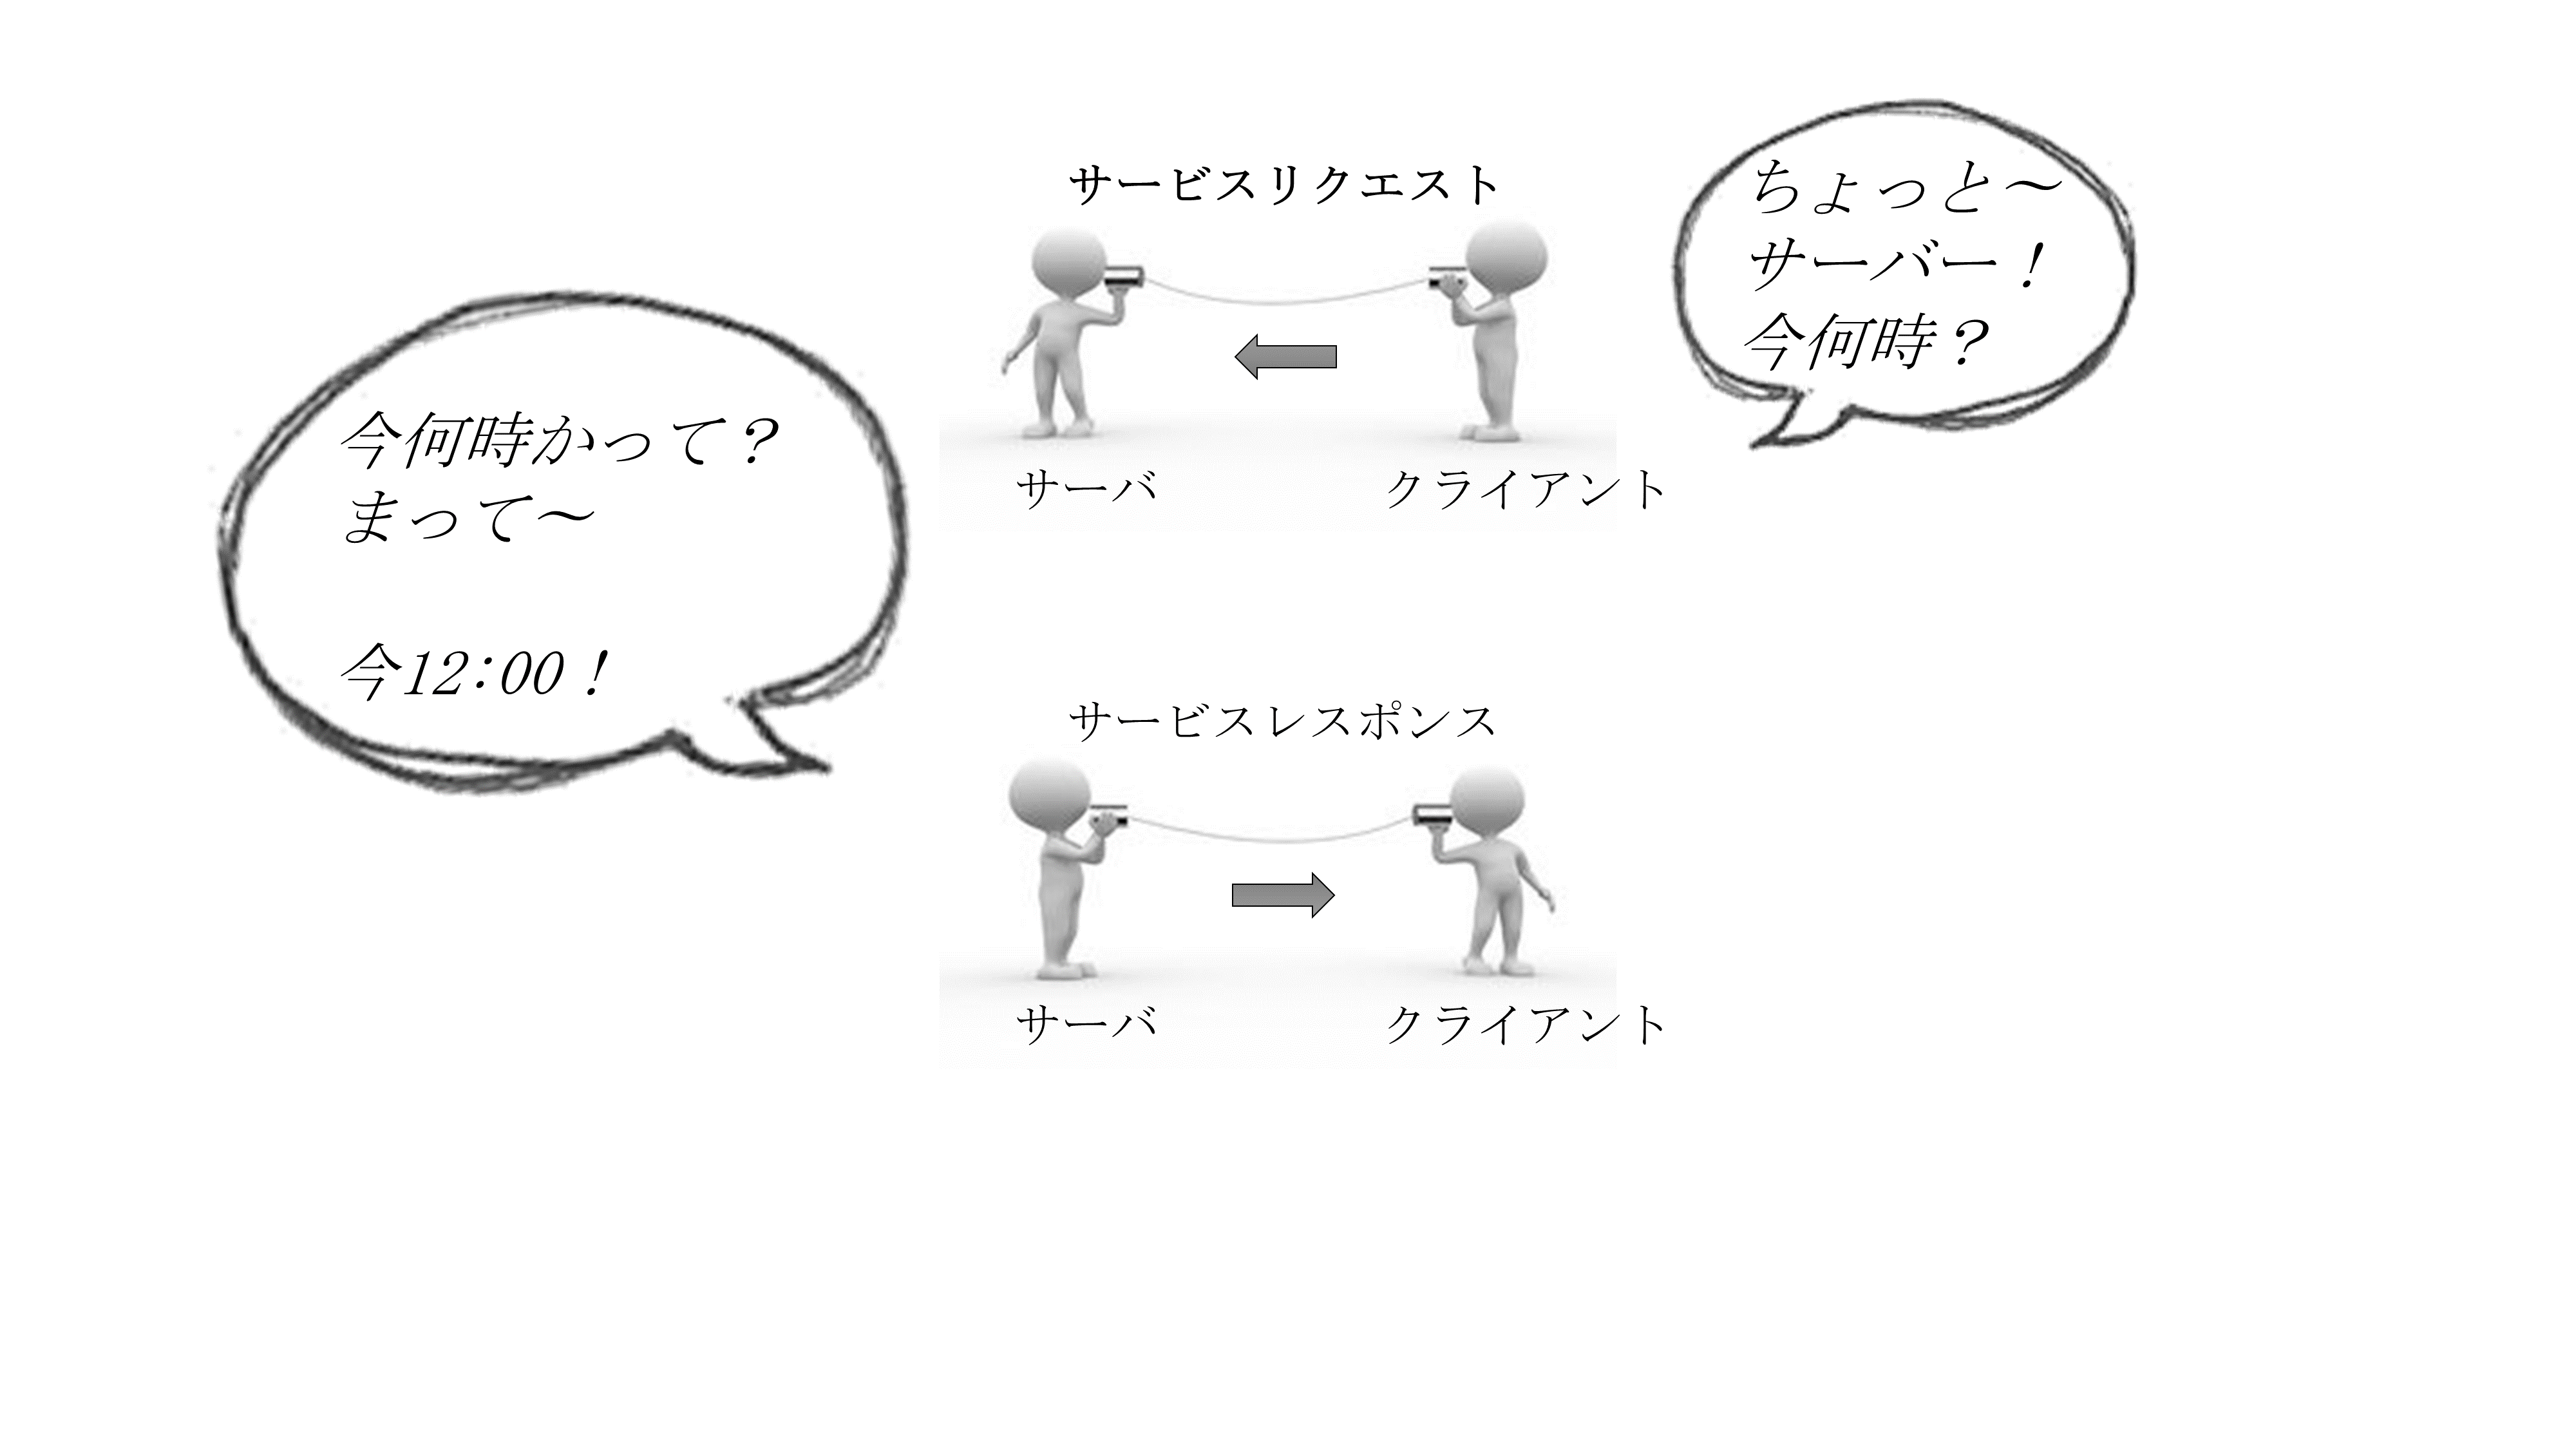
\includegraphics[width=\columnwidth]{pictures/chapter3/pic_03_02.png}
  \caption{サービスメッセージ通信}
\end{figure}

%-------------------------------------------------------------------------------
\subsection{マスターによる接続管理}
配信者、購読者、サービスサーバ、サービスクライアントは、一般にそれぞれ異なるノードの中に存在する。従って、これらのノードがメッセージ通信をするには、ノードを接続する必要がある。このノード間の接続を管理するのがマスター注3である。マスターは、ノードの名前、トピックやサービスの名前、URIアドレスとポート、パラメータなどの情報を管理している。ノードは、生成と同時にマスターに情報を登録し、マスターを介して接続先のノードの情報を得る。その後、ノードとノードが直接接続してメッセージ通信を行う。
図3-3にノード間のメッセージ通信の仕組みを示す。

\begin{figure}[htp]
  \centering
  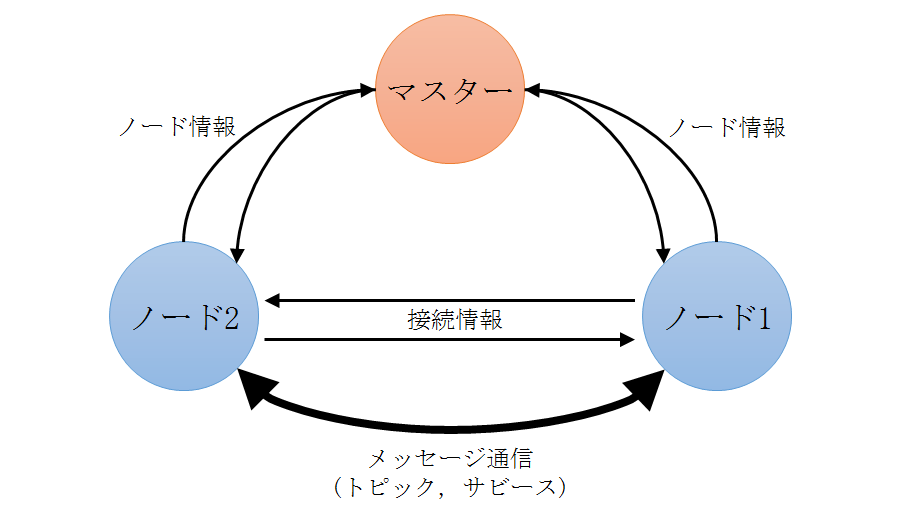
\includegraphics[width=\columnwidth]{pictures/chapter3/pic_03_03.png}
  \caption{メッセージ通信}
\end{figure}

マスターは、ノードの情報を管理し、各ノードは、必要に応じて他のノードと接続、メッセージ通信を行う。以下では、最も重要なマスター、ノード、トピック注4、サービス注5、メッセージ注6間の処理の流れについて、より詳しく説明する。

%-------------------------------------------------------------------------------
\subsection{マスターの実行}

ROSの通信の使用にあたり、ノード間のメッセージ通信の接続情報を管理するマスターを最初に実行する必要がある。ROSマスターは、roscoreコマンドにより実行され、リモートプロシージャコール(RPC)の一種であるXMLRPCを用いてサーバを動作させる。マスターは、ノード間の接続のために、ノードの名前、トピックとサービスの名前、メッセージの形式、URIアドレスとポートを登録し、他のノードから問い合わせがあったときに、必要なノードの情報を送信する。

\begin{lstlisting}[language=ROS]
$ roscore
\end{lstlisting}

\begin{figure}[htp]
  \centering
  
\includegraphics[width=\columnwidth]{pictures/chapter3/pic_03_04.png}
  \caption{マスターのみを起動した状態}
\end{figure}

%-------------------------------------------------------------------------------
\subsection{購読者(subscriber node)の実行}
購読者ノードは、rosrun又はroslaunchコマンドにより実行される。購読者ノードは、実行時に、マスターに自分の購読者ノード名、購読しようとするトピック名、メッセージの形式、URIアドレスとポートを登録する。この時、図3-5のように、マスターと購読者ノードはXMLRPCを利用して通信する。

\begin{lstlisting}[language=ROS]
$ rosrun PACKAGE_NAME NODE_NAME
$ roslaunch PACKAGE_NAME LAUNCH_NAME
\end{lstlisting}

\begin{figure}[htp]
  \centering
  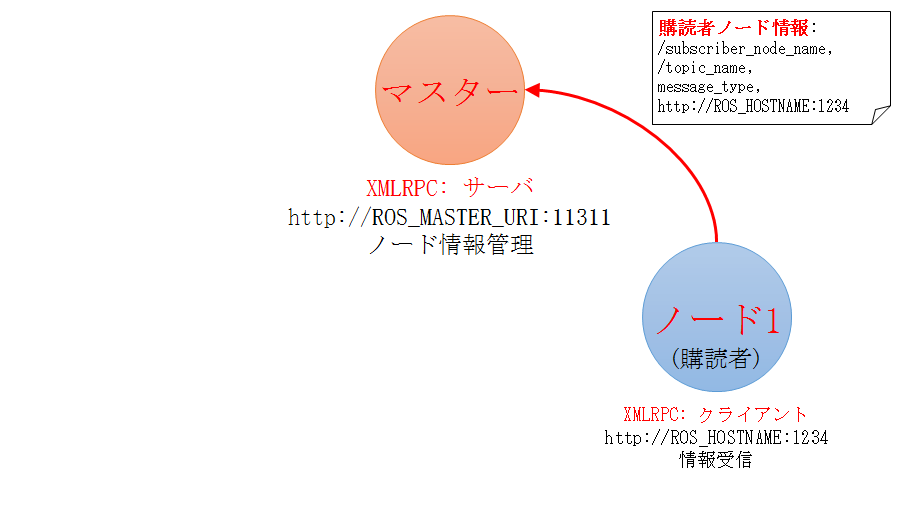
\includegraphics[width=\columnwidth]{pictures/chapter3/pic_03_05.png}
  \caption{購読者ノードの実行}
\end{figure}

%-------------------------------------------------------------------------------
\subsection{配信者ノード(publisher node)の実行}
配信者ノードは、購読者ノードと同様に、rosrun又はroslaunchコマンドにより実行される。配信者ノードは、実行時に、マスターに自分の配信者ノード名、配信しようとするトピック名、メッセージの形式、URIアドレスとポートを登録する。この時、図3-6のように、マスターと配信者ノードはXMLRPCを利用して通信する。

\begin{figure}[htp]
  \centering
  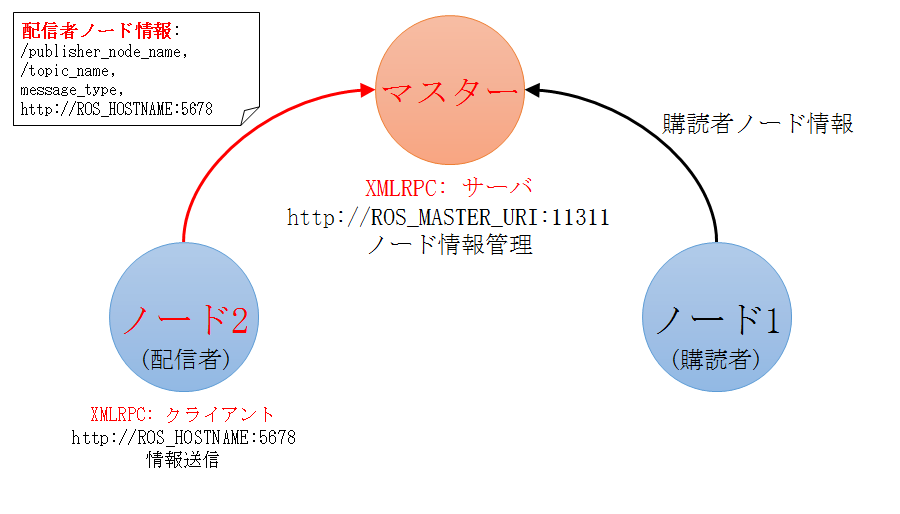
\includegraphics[width=\columnwidth]{pictures/chapter3/pic_03_06.png}
  \caption{配信者ノードの実行}
\end{figure}

%-------------------------------------------------------------------------------
\subsection{購読者ノードへの配信者情報の通知}
マスターは、購読者ノードに購読者が接続したい配信者ノード名やトピック名などの情報を送信する。図3-7のように、マスターと購読者ノードはXMLRPCを利用して通信する。

\begin{figure}[htp]
  \centering
  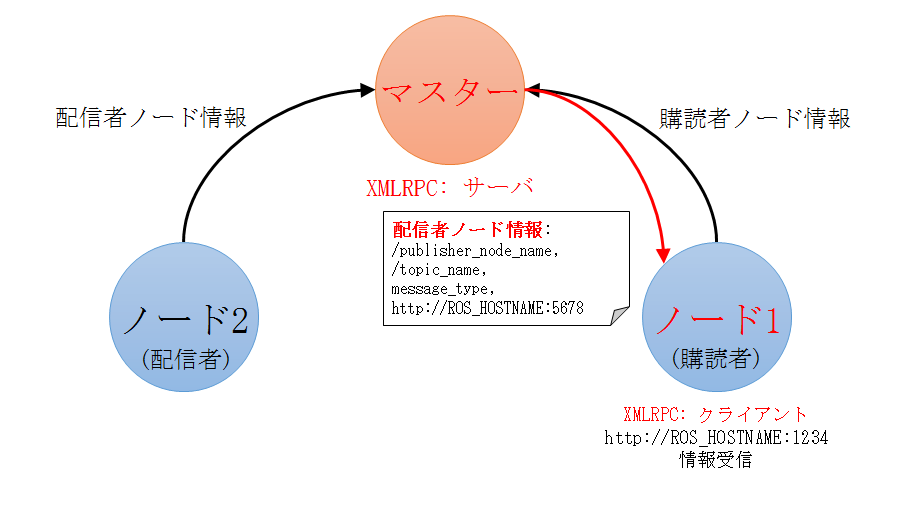
\includegraphics[width=\columnwidth]{pictures/chapter3/pic_03_07.png}
  \caption{購読者へ配信者ノードへの情報の通知}
\end{figure}

%-------------------------------------------------------------------------------
\subsection{購読者ノードの接続要請}
購読者ノードは、マスターから受信した配信者の情報に基づいて、配信者ノードに直接接続を要請する。この時に送信される情報には、自分の購読者ノード名、トピック名、メッセージ方式が含まれる。図3-8のように、配信者ノードと購読者ノードはXMLRPCを利用して通信する。

\begin{figure}[htp]
  \centering
  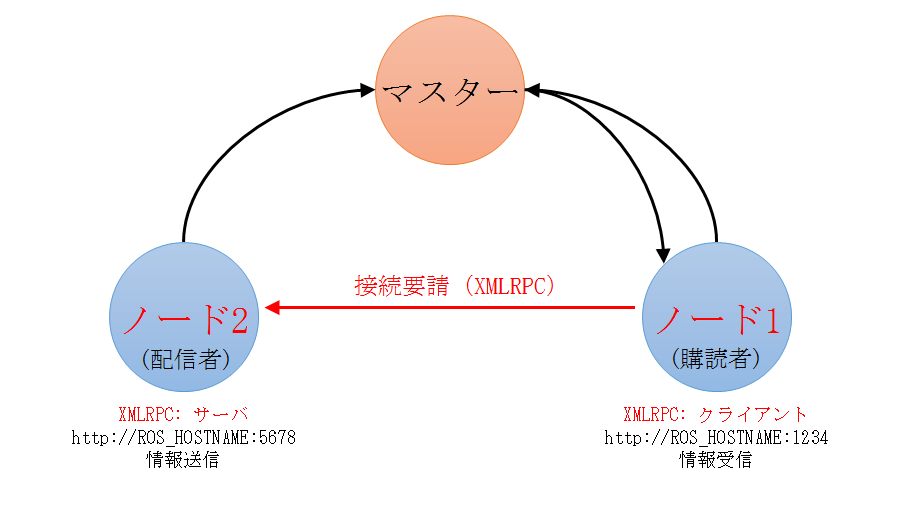
\includegraphics[width=\columnwidth]{pictures/chapter3/pic_03_08.png}
  \caption{配信者ノードに接続要請}
\end{figure}

%-------------------------------------------------------------------------------
\subsection{配信者ノードの接続応答}
配信者ノードは、購読者ノードの接続要請への応答として、自身のURIアドレスとポートを送信する。図3-9のように、配信者ノードと購読者ノードはXMLRPCを利用して通信する。

\begin{figure}[htp]
  \centering
  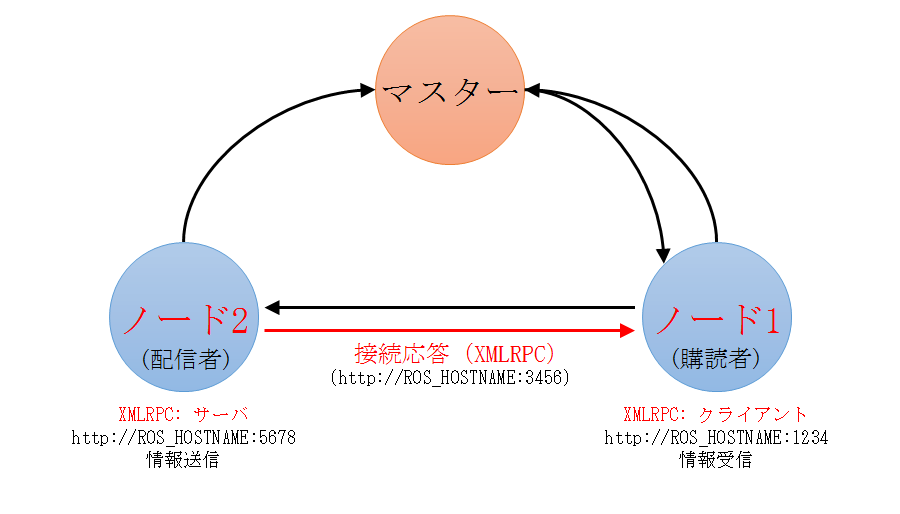
\includegraphics[width=\columnwidth]{pictures/chapter3/pic_03_09.png}
  \caption{配信者ノードの接続応答}
\end{figure}

%-------------------------------------------------------------------------------
\subsection{TCP接続}
購読者ノードはTCPROSを用いて、配信者ノードに対するクライアントを生成し、配信者ノードと直接接続する。図3-10のように、購読者ノードと配信者ノード間はTCP/IP方式であるTCPROSを利用して通信する。

\begin{figure}[htp]
  \centering
  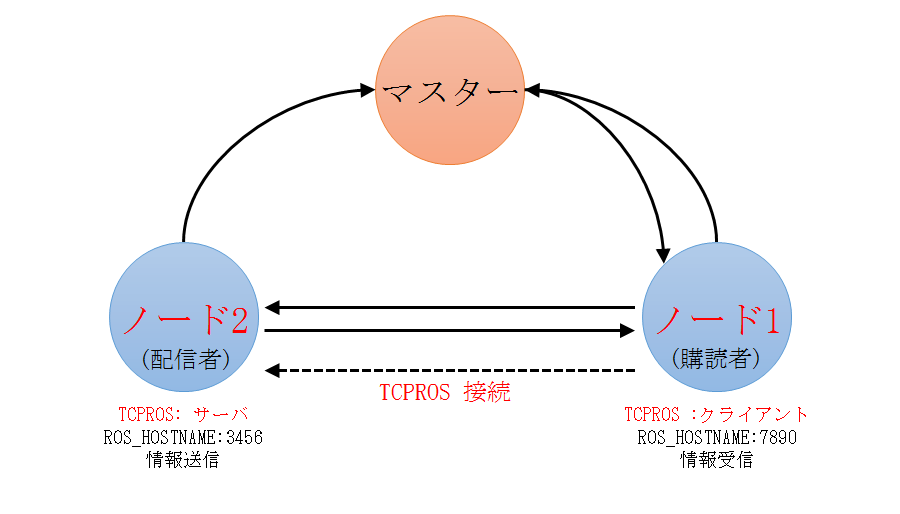
\includegraphics[width=\columnwidth]{pictures/chapter3/pic_03_10.png}
  \caption{購読者ノードと配信者ノードの接続}
\end{figure}

%-------------------------------------------------------------------------------
\subsection{トピックメッセージの送信}
配信者ノードは、購読者ノードにトピックメッセージを送信する。ノード間の通信は、TCPROSを使用する。

\begin{figure}[htp]
  \centering
  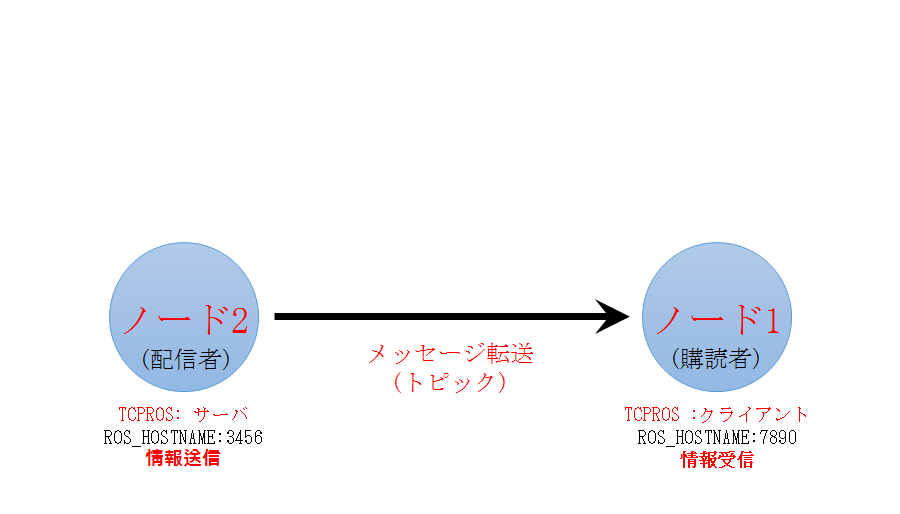
\includegraphics[width=\columnwidth]{pictures/chapter3/pic_03_11.png}
  \caption{トピックメッセージ通信}
\end{figure}

%-------------------------------------------------------------------------------
\subsection{サービスクライアントとサービスサーバによるサービスメッセージ通信}
ここまでは、メッセージ通信のうち、トピックメッセージ通信について学んだ。トピックメッセージ通信では、配信者や購読者が停止していなければ、メッセージを連続して配信し、購読する。
一方、ここからは、もうひとつのメッセージ通信であるサービスメッセージ通信について学んでいこう。サービスメッセージ通信はサービスクライアントとサービスサーバ間で行われる。

\begin{itemize}
\item サービスクライアント:サービスをリクエストする。
\item サービスサーバ:サービスのリクエストを受けて定められた処理を実行し、その結果をレスポンスする。
\end{itemize}
サービスサーバとクライアントの接続は、配信者ノードと購読者ノード間の接続と同様にTCPROS接続である。しかし、サービスメッセージ通信はトピックメッセージ通信とは異なり、1回限り接続して、リクエストとレスポンスを行い、その後お互いの接続を切断する。再度通信するときは、再び接続から始めなければならない。

\begin{figure}[htp]
  \centering
  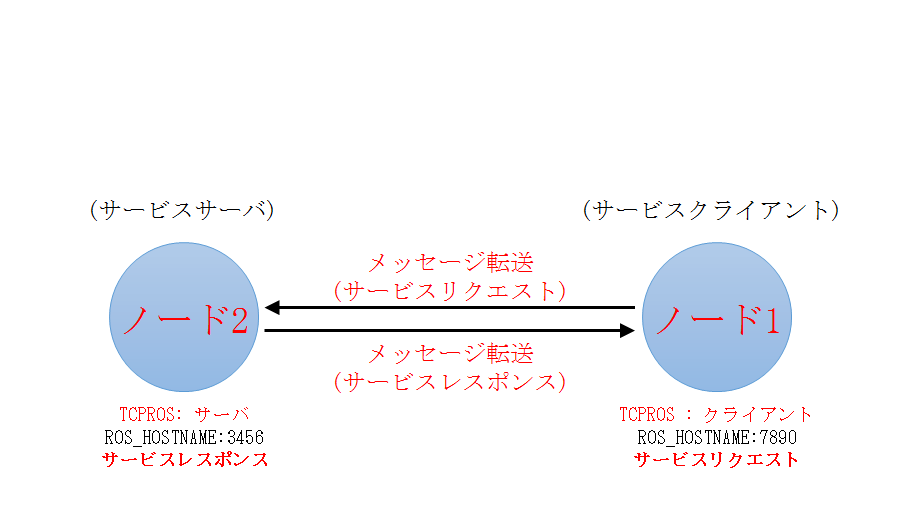
\includegraphics[width=\columnwidth]{pictures/chapter3/pic_03_12.png}
  \caption{サービスメッセージ通信}
\end{figure}

%-------------------------------------------------------------------------------
\subsection{メッセージ通信の例}
2章では、turtlesimを利用して、ROSの動作をテストした。この例でもマスターと2つのノードが使用され、両方のノードが「/turtle1/cmd\_vel」というトピックを利用してメッセージ通信を行った。上記のROSにおける通信の手順に照らし合わせると、これは図3-13のように理解できる。

\begin{figure}[htp]
  \centering
  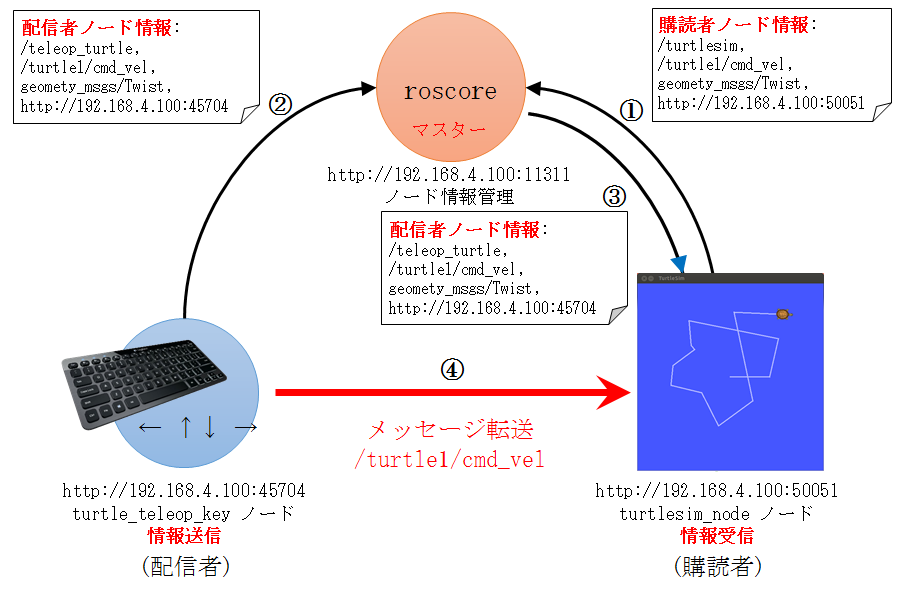
\includegraphics[width=\columnwidth]{pictures/chapter3/pic_03_13.png}
  \caption{turtlesim におけるメッセージ通信の例}
\end{figure}

%-------------------------------------------------------------------------------
\section{ROSファイルシステム}\index{ROSファイルシステム}
OSのファイルシステムは、ROSのインストールフォルダとユーザー作業フォルダに分けられる。
ROSのデスクトップバージョンをインストールすると、/optフォルダにrosという名前でインストールフォルダが作成され、その中にroscoreを含む重要なユーティリティとrqt、RViz、ロボット関連のライブラリ、シミュレーション、ナビゲーションなどが置かれる。ユーザーが/optフォルダのファイルを触れることはほとんどない。もしバイナリファイルとして公式配布されているパッケージを変更しようとする場合は、「sudo apt-get install ros-indigo-xxx」などのパッケージのインストールコマンドではなく、直接、元のソースがあるリポジトリアドレスを確認し、「cd ~/catkin\_ws/src」 として作業フォルダ内のソースフォルダに移動し、「git clone [リポジトリアドレス]」のようにソースをコピーしてビルドすればよい。
ユーザー作業フォルダは、ユーザーが指定した任意の場所に作成できるが、特に問題がなければ、Linuxのユーザーフォルダに「~/catkin\_ws/」(「~/」は、Linux上で「/home/ユーザー名」に対応するフォルダ)を作成して利用する。
続いて、ROSのインストールフォルダとユーザー作業フォルダについて、さらに詳しく説明する。

%-------------------------------------------------------------------------------
\subsection{ROSのインストールフォルダ}\index{ROSのインストールフォルダ}
ROSは、「/opt/ros/[バージョン名]」フォルダにインストールされている。例えば、Indigoバージョンをインストールした場合、ROSがインストールされたフォルダは、次のとおりである。

\begin{itemize}
\item ROSのインストールフォルダ: /opt/ros/indigo
\end{itemize}

ROSのインストールフォルダである「/opt/ros/indigo」フォルダは、図3-14のように、「bin」、「etc」、「include」、「lib」、「share」などのフォルダと、環境設定ファイルで構成されている。

\begin{figure}[htp]
  \centering
  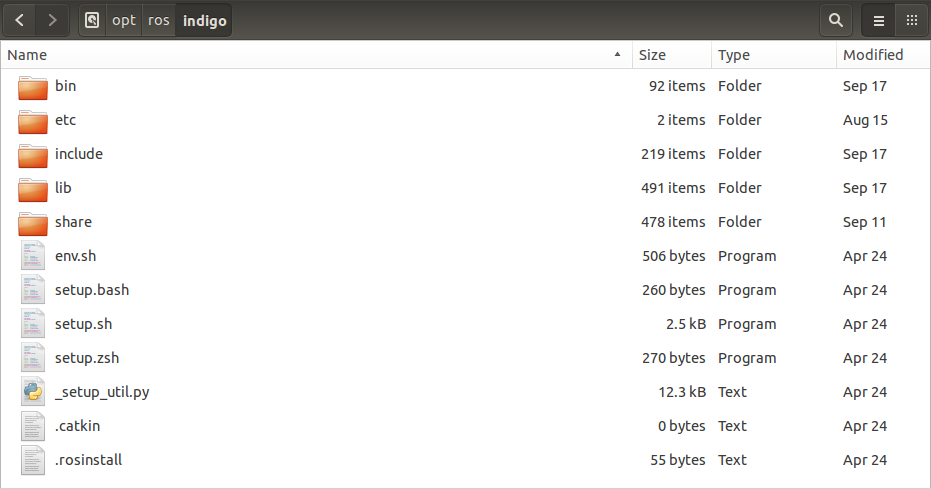
\includegraphics[width=\columnwidth]{pictures/chapter3/pic_03_14.png}
  \caption{ROSファイルの構成}
\end{figure}

各フォルダの詳細は、次のとおりである。

\begin{itemize}
\item /bin    実行可能なバイナリファイル
\item /etc    ROSとcatkin関連の設定ファイル
\item /include  ヘッダーファイル
\item /lib    ライブラリファイル
\item /share  ROSパッケージ
\item env.*   環境設定ファイル
\item setup.* 環境設定ファイル
\end{itemize}

%-------------------------------------------------------------------------------
\subsection{ユーザー作業フォルダ}\index{ユーザー作業フォルダ}

ユーザー作業フォルダは、ユーザーが指定した任意の場所に作成することができるが、本書では、ユーザー作業フォルダとして「~/catkin\_ws/」、あるいは「/home/ユーザー名/catkin\_ws」を使用する。例えば、ユーザー名が「irvs」でcatkinフォルダ名を「catkin\_ws」とすると、ユーザー作業フォルダは以下のフォルダとなる。

\begin{itemize}
\item ユーザー作業フォルダ: /home/irvs/catkin\_ws/
\end{itemize}

ユーザー作業フォルダは、ユーザーが作成したパッケージや、他の開発者が作成し、公開しているパッケージを保存し、ビルドする場所である。ユーザーは、ROSに関連するほとんどの作業を、このフォルダ内で行う。

%-------------------------------------------------------------------------------
\subsubsection{ファイルの構成}
ユーザー作業フォルダは、図3-15のようにbuild、devel、srcの3つのフォルダで構成されている。

\begin{figure}[htp]
  \centering
  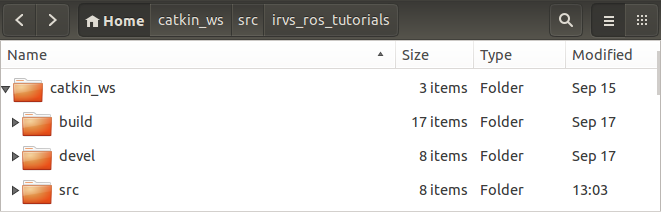
\includegraphics[width=\columnwidth]{pictures/chapter3/pic_03_15.png}
  \caption{catkin workspaceのファイル構成}
\end{figure}

それぞれのフォルダの詳細は、次のとおりである。

\begin{itemize}
\item /build  ビルド関連ファイル
\item /devel  msg又はsrvのヘッダーファイルとユーザーパッケージのライブラリ、実行ファイル
\item /src    ユーザーパッケージ
\end{itemize}

%-------------------------------------------------------------------------------
\subsubsection{ユーザーパッケージ}
「src」フォルダは、ユーザーのソースコードを置くフォルダである。このフォルダにユーザーが開発したROSパッケージや他のユーザーが開発したパッケージを保存する。図3-16は、著者が作成したirvs\_ros\_tutorialsというパッケージを展開した後の状態である。

\begin{figure}[htp]
  \centering
  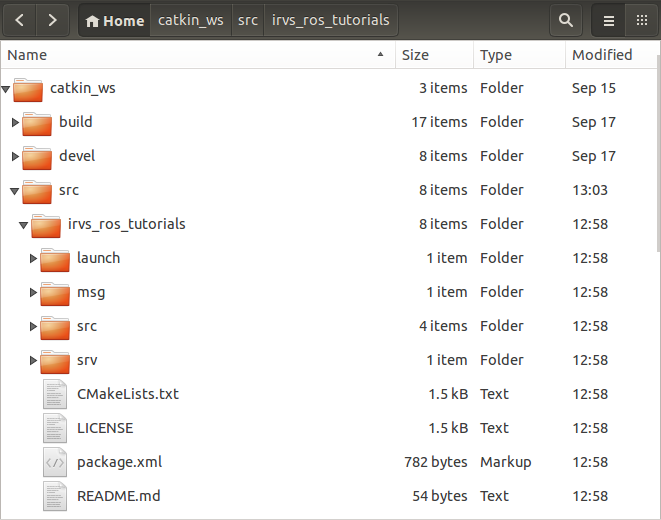
\includegraphics[width=\columnwidth]{pictures/chapter3/pic_03_16.png}
  \caption{ユーザーパッケージのファイル構成}
\end{figure}

\begin{itemize}
\item /include    ヘッダーファイル
\item /launch   roslaunchに使用されるlaunchファイル
\item /node     rospy用スクリプト
\item /msg      メッセージのファイル
\item /src      ソースコードファイル
\item /srv      サービスファイル
\item CMakeLists.txt  ビルドの設定ファイル
\item package.xml   パッケージの設定ファイル
\end{itemize}

%-------------------------------------------------------------------------------
\section{ROSビルドシステム}\index{ROSビルドシステム}

ROSのビルドシステムは、ROSパッケージをマルチプラットフォームで開発するため、基本的にはCMake(Cross Platform Make)注7を利用している。catkinビルドシステムは、CMakeをROSに合わせて改良したものであり、CMakeと同様にパッケージのフォルダ内のCMakeLists.txtファイルにビルド環境を記述している。Make注8がUnix系を主な対象としているのとは異なり、CMakeは、Unix系のLinux、BSD、Mac OS Xだけでなく、Windows系にも対応している。また、マイクロソフトのVisual Studioもサポートしており、QT注9の開発にも容易に適用できる。さらに、catkinビルドシステムは、ROSに関連するビルド、パッケージ管理、依存関係パッケージの自動インストールなども容易に実行できる。

%-------------------------------------------------------------------------------
\subsection{パッケージの作成}
ROSパッケージを作成するコマンドは次のとおりである。

\begin{lstlisting}[language=ROS]
$ catkin_create_pkg %*[パッケージ名] [依存するパッケージ1]…[依存するパッケージn]*)
\end{lstlisting}



「catkin\_create\_pkg」コマンドを実行すると、catkinビルドシステムに必要なCMakeLists.txtとpackage.xmlを含む空のパッケージフォルダが作成される。実際に簡単なパッケージを作成してみよう。まず、次のコマンドでユーザー作業フォルダの「src」フォルダに移動する。

\begin{lstlisting}[language=ROS]
$ cd ~/catkin_ws/src
\end{lstlisting}

ここで作成するパッケージの名前は「my\_first\_ros\_pkg」である。 ROSのパッケージ名には、通常はすべて小文字を使用し、スペースは使用できない。またハイフン(-)ではなくアンダースコア(\_)を使用し、各単語を続ける。ROSプログラミングにおけるコーディングスタイルと名前の規則については、関連ページ注10,11,12を参照してほしい。
では、次のコマンドでmy\_first\_ros\_pkgという名前のパッケージを作成しよう。

\begin{lstlisting}[language=ROS]
$ catkin_create_pkg my_first_ros_pkg std_msgs roscpp
\end{lstlisting}

上記のコマンドでは、依存するパッケージ「std\_msgs」と「roscpp」をオプションとして記述している。これは作成するパッケージでは、ROSの標準的なメッセージパッケージstd\_msgsとC/C++を使用するためのクライアントライブラリroscppを使用するため、パッケージの作成に先立ってこれらをインストールしておく必要があることを意味する。依存するパッケージの設定は、上記のようにパッケージの作成時に指定する方法もあるが、生成されたフォルダ内の「package.xml」に後から直接記述してもよい。
パッケージを作成すると、「~/catkin\_ws/src」の下に「my\_first\_ros\_pkg」というパッケージのフォルダが作成され、その中にROSパッケージが備えるべき基本的なフォルダと、CMakeLists.txtとpackage.xmlファイルが生成される。次のように「ls」コマンドや、UbuntuのGUIベースのNautilusを利用して、パッケージの内部を見てみよう。

\begin{lstlisting}[language=ROS]
$ ls
include
src
CMakeLists.txt
package.xml
\end{lstlisting}

\begin{figure}[htp]
  \centering
  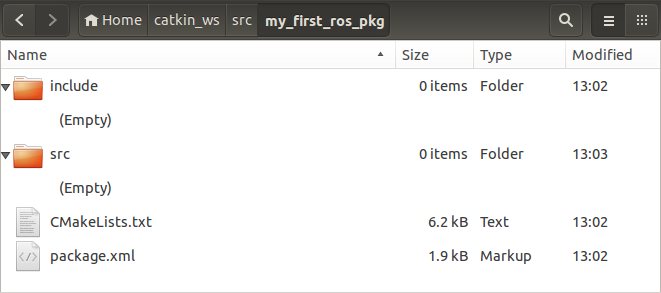
\includegraphics[width=\columnwidth]{pictures/chapter3/pic_03_17.png}
  \caption{自動生成されたファイルとフォルダ}
\end{figure}

 %-------------------------------------------------------------------------------
 \subsection{パッケージ設定ファイル(package.xml)の変更}
ROSのパッケージの設定ファイルであるpackage.xmlは、パッケージの名前、著作者、ライセンス、依存性パッケージなどのパッケージの情報を、XMLファイルとして保存している。作成直後のpackage.xmlファイルは、以下の通りである。

ファイル名:package.xml

\begin{lstlisting}[language=ROS]
<?xml version="1.0"?>
<package>
<name>my_first_ros_pkg</name>
<version>0.0.0</version>
<description>The my_first_ros_pkg package</description>

<!-- One maintainer tag required, multiple allowed, one person per tag -->
<!-- Example:  -->

<!-- <maintainer email="jane.doe@example.com">Jane Doe</maintainer> -->
<maintainer email="rt@todo.todo">rt</maintainer>

<!-- One license tag required, multiple allowed, one license per tag -->
<!-- Commonly used license strings: -->
<!-- BSD, MIT, Boost Software License, GPLv2, GPLv3, LGPLv2.1, LGPLv3 -->
<license>TODO</license>

<!-- Url tags are optional, but mutiple are allowed, one per tag -->
<!-- Optional attribute type can be: website, bugtracker, or repository -->
<!-- Example: -->
<!-- <url type="website">http://wiki.ros.org/my_first_ros_pkg</url> -->

<!-- Author tags are optional, mutiple are allowed, one per tag -->
<!-- Authors do not have to be maintianers, but could be -->
<!-- Example: -->
<!-- <author email="jane.doe@example.com">Jane Doe</author> -->

<!-- The *_depend tags are used to specify dependencies -->
<!-- Dependencies can be catkin packages or system dependencies -->
<!-- Examples: -->
<!-- Use build_depend for packages you need at compile time: -->
<!-- <build_depend>message_generation</build_depend> -->
<!-- Use buildtool_depend for build tool packages: -->
<!-- <buildtool_depend>catkin</buildtool_depend> -->
<!-- Use run_depend for packages you need at runtime: -->
<!-- <run_depend>message_runtime</run_depend> -->
<!-- Use test_depend for packages you need only for testing: -->
<!-- <test_depend>gtest</test_depend> -->
<buildtool_depend>catkin</buildtool_depend>
<build_depend>roscpp</build_depend>
<build_depend>std_msgs</build_depend>
<run_depend>roscpp</run_depend>
<run_depend>std_msgs</run_depend>

<!-- The export tag contains other, unspecified, tags -->
<export>
<!-- You can specify that this package is a metapackage here: -->
<!-- <metapackage/> -->
<!-- Other tools can request additional information be placed here -->
</export>
</package>
\end{lstlisting}

各構文について説明する。

\begin{itemize}
\item <? xml> ドキュメントの文法を定義する構文で、以下の内容は、xmlバージョン1.0であることを意味する。
\item <package> この構文から</package>までがROSパッケージの設定部分である。
\item <name> パッケージの名前である。パッケージを作成するときに入力したパッケージ名が使用される。他のオプションも同じであるが、パッケージ名はユーザーが必要なときにいつでも変更することができる。ただし、後で説明するCMakeLists.txtファイルの「project」部分と一致していなければならない。
\item <version> パッケージのバージョンである。自由に指定することができる。
\item <description> パッケージの簡単な説明である。
\item <maintainer> パッケージマネージャの連絡先を記載する。
\item <license> ライセンスを記載する。 BSD、MIT、GPLv3、LGPLv3などを記載すればよい。
\item <url> パッケージを説明しているWebページまたはバグ管理、ストレージなどのアドレスを記載する。種類に応じてtypeにはwebsite、bugtracker、repositoryを記載すればよい。
\item <author> パッケージの開発に参加した開発者を示す。複数の開発者が参加した場合は、次の行に<author>タグを使用して、追加すれば良い。
\item <buildtool\_depend> ビルドシステムの依存関係を記述する。現在はcatkinビルドシステムを利用しているのでcatkinと記述する。
\item <build\_depend> パッケージをビルドするときに依存するパッケージの名前を書く。
\item <run\_depend> パッケージを実行するときに依存するパッケージの名前を書く。
\item <test\_depend> パッケージをテストするときに依存するパッケージの名前を書く。
\item <export> ROSで明示していないタグ名を使用するときに使われる。ただし、使用頻度は低い。
\item <metapackage> exportタグ内で使用するタグであり、現在のパッケージがメタパッケージであれば、ここで宣言する。
\end{itemize}

上述した作成直後のファイルに必要な情報を追加し、不要な行を削除したパッケージ設定ファイル(package.xml)の一例を示す。

ファイル名:package.xml

\begin{lstlisting}[language=XML]
<?xml version="1.0"?>
<package>
<name>my_first_ros_pkg</name>
<version>0.0.1</version>
<description>The my_first_ros_pkg package</description>

<maintainer email = "aaa@bbb.jp">Anonymous</maintainer>

<license>BSD</license>
<url type = "website"> http://irvs.github.io/ros_tms/</url>
<url type="repository">https://github.com/irvs/irvs_ros_tutorials.git</url>
<author email = "aaa@bbb.jp">Anonymous</author>

<buildtool_depend>catkin</buildtool_depend>

<build_depend>std_msgs</build_depend>
<build_depend>roscpp</build_depend>

<run_depend>std_msgs</run_depend>
<run_depend>roscpp</run_depend>

<export>
</export>
</package>
\end{lstlisting}

%-------------------------------------------------------------------------------
\subsection{ビルド設定ファイル(CMakeLists.txt)の変更}
ROSのビルドシステムであるcatkinでは、パッケージのフォルダ内のCMakeLists.txtファイルにビルドの環境を記述している。このCMakeLists.txtファイルには、作成するパッケージ名、依存パッケージ名、実行可能ファイル名などを設定する。作成直後のCMakeLists.txtファイルは、以下の通りである。

ファイル名:CMakeLists.txt

\begin{lstlisting}[language=make]
cmake_minimum_required(VERSION 2.8.3)
project(my_first_ros_pkg)

## Find catkin macros and libraries
## if COMPONENTS list like find_package(catkin REQUIRED COMPONENTS xyz)
## is used, also find other catkin packages
find_package(catkin REQUIRED COMPONENTS roscpp std_msgs)

## System dependencies are found with CMake's conventions
# find_package(Boost REQUIRED COMPONENTS system)

## Uncomment this if the package has a setup.py. This macro ensures
## modules and global scripts declared therein get installed
## See http://ros.org/doc/api/catkin/html/user_guide/setup_dot_py.html
# catkin_python_setup()

################################################
## Declare ROS messages, services and actions ##
################################################

## To declare and build messages, services or actions from within this
## package, follow these steps:
## * Let MSG_DEP_SET be the set of packages whose message types you use in
##  your messages/services/actions (e.g. std_msgs, actionlib_msgs, ...).
## * In the file package.xml:
##  * add a build_depend and a run_depend tag for each package in MSG_DEP_SET
##  * If MSG_DEP_SET isn't empty the following dependencies might have been
##  pulled in transitively but can be declared for certainty nonetheless:
##  * add a build_depend tag for "message_generation"
##  * add a run_depend tag for "message_runtime"
## * In this file (CMakeLists.txt):
##  * add "message_generation" and every package in MSG_DEP_SET to
##  find_package(catkin REQUIRED COMPONENTS ...)
##  * add "message_runtime" and every package in MSG_DEP_SET to
##  catkin_package(CATKIN_DEPENDS ...)
##  * uncomment the add_*_files sections below as needed
##  and list every .msg/.srv/.action file to be processed
##  * uncomment the generate_messages entry below
##  * add every package in MSG_DEP_SET to generate_messages(DEPENDENCIES ...)

## Generate messages in the 'msg' folder
# add_message_files(
# FILES
# Message1.msg
# Message2.msg
# )

## Generate services in the 'srv' folder
# add_service_files(
# FILES
# Service1.srv
# Service2.srv
# )

## Generate actions in the 'action' folder
# add_action_files(
# FILES
# Action1.action
# Action2.action
# )

## Generate added messages and services with any dependencies listed here
# generate_messages(
# DEPENDENCIES
# std_msgs
# )

###################################
## catkin specific configuration ##
###################################
## The catkin_package macro generates cmake config files for your package
## Declare things to be passed to dependent projects
## INCLUDE_DIRS: uncomment this if you package contains header files
## LIBRARIES: libraries you create in this project that dependent projects also need
## CATKIN_DEPENDS: catkin_packages dependent projects also need
## DEPENDS: system dependencies of this project that dependent projects also need catkin_package(
#  INCLUDE_DIRS include
#  LIBRARIES my_first_ros_pkg
#  CATKIN_DEPENDS roscpp std_msgs
#  DEPENDS system_lib
)

###########
## Build ##
###########

## Specify additional locations of header files
## Your package locations should be listed before other locations
# include_directories(include) include_directories(
${catkin_INCLUDE_DIRS}
)

## Declare a cpp library
# add_library(my_first_ros_pkg
# src/${PROJECT_NAME}/my_first_ros_pkg.cpp
# )

## Declare a cpp executable
# add_executable(my_first_ros_pkg_node src/my_first_ros_pkg_node.cpp)

## Add cmake target dependencies of the executable/library
## as an example, message headers may need to be generated before nodes
# add_dependencies(my_first_ros_pkg_node my_first_ros_pkg_generate_messages_cpp)

## Specify libraries to link a library or executable target against
# target_link_libraries(my_first_ros_pkg_node
# ${catkin_LIBRARIES}
# )

#############
## Install ##
#############

# all install targets should use catkin DESTINATION variables
# See http://ros.org/doc/api/catkin/html/adv_user_guide/variables.html

## Mark executable scripts (Python etc.) for installation
## in contrast to setup.py, you can choose the destination
# install(PROGRAMS
# scripts/my_python_script
# DESTINATION ${CATKIN_PACKAGE_BIN_DESTINATION}
# )

## Mark executables and/or libraries for installation
# install(TARGETS my_first_ros_pkg my_first_ros_pkg_node
# ARCHIVE DESTINATION ${CATKIN_PACKAGE_LIB_DESTINATION}
# LIBRARY DESTINATION ${CATKIN_PACKAGE_LIB_DESTINATION}
# RUNTIME DESTINATION ${CATKIN_PACKAGE_BIN_DESTINATION}
# )

## Mark cpp header files for installation
# install(DIRECTORY include/${PROJECT_NAME}/
# DESTINATION ${CATKIN_PACKAGE_INCLUDE_DESTINATION}
# FILES_MATCHING PATTERN "*.h"
# PATTERN ".svn" EXCLUDE
# )

## Mark other files for installation (e.g. launch and bag files, etc.)
# install(FILES
# # myfile1
# # myfile2
# DESTINATION ${CATKIN_PACKAGE_SHARE_DESTINATION}
# )

#############
## Testing ##
#############

## Add gtest based cpp test target and link libraries
# catkin_add_gtest(${PROJECT_NAME}-test test/test_my_first_ros_pkg.cpp)
# if(TARGET ${PROJECT_NAME}-test)
# target_link_libraries(${PROJECT_NAME}-test ${PROJECT_NAME})
# endif()

## Add folders to be run by python nosetests
# catkin_add_nosetests(test)
\end{lstlisting}

ビルド設定ファイル(CMakeLists.txt)の各オプションは、次の通りである。

\begin{lstlisting}[language=make]
cmake_minimum_required(VERSION 2.8.3)
\end{lstlisting}

オペレーティングシステムにインストールされているcmakeの最低限必要なバージョンである。この例では2.8.3バージョンと記載されているので、これ以前のバージョンのcmakeを利用している場合は、cmakeを更新する必要がある。

\begin{lstlisting}[language=make]
project(my_first_ros_pkg)
\end{lstlisting}

パッケージの名前である。「package.xml」で入力したパッケージ名をそのまま使用する。もしpackage.xmlの<name>タグに記述したパッケージ名と異なる場合は、ビルドするときにエラーが発生する。

\begin{lstlisting}[language=make]
find_package(catkin REQUIRED COMPONENTS roscpp std_msgs)
\end{lstlisting}

catkinビルドをするときに必要なコンポーネントパッケージ、すなわち依存パッケージを指定する。この例では、依存パッケージとしてroscppとstd\_msgsが指定されている。ここで指定されたパッケージが存在しない場合、ビルドするときにエラーが表示される。

\begin{lstlisting}[language=make]
find_package(Boost REQUIRED COMPONENTS system)
\end{lstlisting}

ROS以外のパッケージまたはライブラリを使用するときの記述方法である。この例では、BoostというC++ライブラリを使用する際、systemというBoostのコンポーネントライブラリがインストールされていなければならないことを意味する。

\begin{lstlisting}[language=make]
catkin_python_setup()
\end{lstlisting}

Pythonを使用する時に設定するオプションである。Pythonのインストールプロセスであるsetup.py注13を呼ぶ。

\begin{lstlisting}[language=make]
add_message_files (FILES
  Message1.msg
  Message2.msg
)
\end{lstlisting}

使用するメッセージファイルを追加するためのオプションである。FILESの後に使用するメッセージファイル(*.msg)を記述しておくと、現在のパッケージフォルダのmsgフォルダ内のmsgファイルを参照し、関連するヘッダーファイルを自動生成する。この例では、Message1.msgとMessage2.msgのメッセージファイルを利用する。

\begin{lstlisting}[language=make]
add_service_files (FILES
  Service1.srv
  Service2.srv
)
\end{lstlisting}

使用するサービスファイルを追加するためのオプションである。 FILESの後に使用するサービスファイル(*.srv)を記述しておくと、現在のパッケージフォルダのsrvフォルダ内のsrvファイルを参照し、関連するヘッダーファイルを自動生成する。この例では、Service1.srvとService2.srvのサービスファイルを利用する。

\begin{lstlisting}[language=make]
generate_messages (DEPENDENCIES std_msgs)
\end{lstlisting}

依存しているメッセージを設定するためのオプションである。この例では、DEPENDENCIESオプションによってstd\_msgsというメッセージパッケージを使用する。

\begin{lstlisting}[language=make]
catkin_package (INCLUDE_DIRS include
     LIBRARIES my_first_ros_pkg
     CATKIN_DEPENDS roscpp std_msgs
     DEPENDS system_lib
)
\end{lstlisting}

catkinビルドオプションである。 INCLUDE\_DIRSではヘッダーファイルの置かれたフォルダを指定し、ここではパッケージフォルダのincludeフォルダを指定している。LIBRARIESでは、「add\_library」で指定したライブラリの保存先フォルダを指定する。このLIBRARIES フォルダは「catkin\_ws/devel/lib」の下に生成される。CATKIN\_DEPENDSはroscppやstd\_msgなど、依存するパッケージを指定し、上の例ではroscppとstd\_msgsが依存していると設定している。DEPENDSはシステム依存のパッケージを記述するための設定である。

\begin{lstlisting}[language=make]
include_directories ($ {catkin_INCLUDE_DIRS})
\end{lstlisting}

インクルードフォルダを指定できるオプションである。この例では、\${catkin\_INCLUDE\_DIRS}と設定されているが、これは生成したパッケージ内のincludeフォルダを意味し、この中のヘッダーファイルを利用する。

\begin{lstlisting}[language=make]
add_library (my_first_ros_pkg src/${PROJECT_NAME}/my_first_ros_pkg.cpp)
\end{lstlisting}

ビルドする際、作成するライブラリを指定する。この例では、src/\${PROJECT\_NAME} /my\_first\_ros\_pkg.cppファイルを参照して、my\_first\_ros\_pkgというライブラリを作成する。

\begin{lstlisting}[language=make]
add_executable (my_first_ros_pkg_node src/my_first_ros_pkg_node.cpp)
\end{lstlisting}

ビルドする際、作成する実行可能ファイルを指定する。この例では、src/my\_first\_ros\_pkg\_node.cppファイルを参照して、my\_first\_ros\_pkg\_nodeという実行ファイルを生成する。

\begin{lstlisting}[language=make]
add_dependencies (my_first_ros_pkg_node my_first_ros_pkg_generate_messages_cpp)
\end{lstlisting}

パッケージをビルドする前に、メッセージのヘッダーファイルを作成する必要がある場合、パッケージのビルド前にメッセージファイルを生成するための設定である。この例では、my\_first\_ros\_pkg\_generate\_messages\_cppとしてmsgやsrv関連ヘッダーファイルを優先的に生成した後で、my\_first\_ros\_pkg\_nodeをビルドする。

\begin{lstlisting}[language=make]
target_link_libraries (my_first_ros_pkg_node
${catkin_LIBRARIES}
)
\end{lstlisting}

my\_first\_ros\_pkg\_nodeを作成する際に、リンクするライブラリを指定するオプションである。
作成直後のファイルから不要な行を削除したビルド設定ファイル(CMakeLists.txt)を示す。

ファイル名:CMakeLists.txt
\begin{lstlisting}[language=make]
cmake_minimum_required(VERSION 2.8.3)
project(my_first_ros_pkg)

find_package(catkin REQUIRED COMPONENTS roscpp std_msgs)

catkin_package( INCLUDE_DIRS include
    CATKIN_DEPENDS roscpp std_msgs
    DEPENDS system_lib
)

include_directories( ${catkin_INCLUDE_DIRS} )

add_executable(hello_world_node src/hello_world_node.cpp) add_dependencies(hello_world_node my_first_ros_pkg_generate_messages_cpp) target_link_libraries(hello_world_node ${catkin_LIBRARIES})
\end{lstlisting}

%-------------------------------------------------------------------------------
\subsection{ソースコードの作成}
上述したCMakelists.txtファイルにおいて、実行ファイルを作成する部分(add\_executable)には次のように記述した。

\begin{lstlisting}[language=ROS]
add_executable (hello_world_node src/hello_world_node.cpp)
\end{lstlisting}

これは、パッケージフォルダのsrcフォルダ内にあるhello\_world\_node.cppソースコードから、hello\_world\_nodeという名前の実行ファイルを生成する設定である。しかし、まだhello\_world\_node.cppというファイルがないので、作成してみよう。
まず、「cd」コマンドで作成したパッケージフォルダ内のソースコードを保存するフォルダ(src)に移動し、hello\_world\_node.cppファイルを生成する。次の例では、geditというエディタを使用したが、sublime text、vim、emacs、nanoなど好きなエディタを利用してかまわない。

\begin{lstlisting}[language=ROS]
$ cd ~/catkin_ws/src/my_first_ros_pkg/src
$ gedit hello_world_node.cpp
\end{lstlisting}

次に、以下のソースコードを作成し、保存する。

ファイル名:hello\_world\_node.cpp

\begin{lstlisting}[language=C++]
#include <ros/ros.h>
#include <std_msgs/String.h>
#include <sstream>

int main(int argc, char **argv)
{
  ros::init(argc, argv, "hello_world_node");
  ros::NodeHandle nh;
  ros::Publisher chatter_pub =
    nh.advertise<std_msgs::String>("say_hello_world", 1000);
  ros::Rate loop_rate(10);
  int count = 0;
  while (ros::ok())
  {
    std_msgs::String msg;
    std::stringstream ss;
    ss << "hello world " << count;
    msg.data = ss.str();
    ROS_INFO("%s", msg.data.c_str());
    chatter_pub.publish(msg);
    ros::spinOnce();
    loop_rate.sleep();
    ++count;
  }
  return 0;
}
\end{lstlisting}

%-------------------------------------------------------------------------------
\subsection{パッケージのビルド}
これで、パッケージをビルドするためのすべての準備作業が終了した。次はユーザー作業フォルダに移動し、catkinビルドを実行しよう。

\begin{lstlisting}[language=ROS]
$ cd ~/catkin_ws && catkin_make
\end{lstlisting}

\begin{exercise}[短縮コマンド]
先に2.2節「ROSの開発環境の構築」で述べたように、「.bashrc」ファイルに「alias cm='cd ~/catkin\_ws \&\& catkin\_make'」と設定しておくと、ターミナルウィンドウで「cm」と入力するだけで、上のコマンドを実行できる。
\end{exercise}

%-------------------------------------------------------------------------------
\subsection{ノードの実行}
これで、パッケージをビルドするためのすべての準備作業が終了した。次はユーザー作業フォルダに移動し、catkinビルドを実行しよう。

エラーがなくビルドが終了したら、「~/catkin\_ws/devel/lib/my\_first\_ros\_pkg」に「hello\_world\_node」という名前のファイルが生成されている。次のステップは、ノードの実行である。ただし、ROSのすべてのノードは、roscoreを実行して初めて利用できるので、必ず先にroscoreを実行しておく必要がある。

\begin{lstlisting}[language=ROS]
$ roscore
\end{lstlisting}

最後に、新しいターミナルウィンドウを開き、次のコマンドでノードを実行してみよう。これは、my\_first\_ros\_pkgという名前のパッケージのhello\_world\_nodeという名前のノードを実行するコマンドである。

\begin{lstlisting}[language=ROS]
$ rosrun my_first_ros_pkg hello_world_node
[INFO] [1423443540.131775283]: hello world 0
[INFO] [1423443540.231826916]: hello world 1
[INFO] [1423443540.331798085]: hello world 2
[INFO] [1423443540.431796634]: hello world 3
[INFO] [1423443540.531808660]: hello world 4
[INFO] [1423443540.631800431]: hello world 5
[INFO] [1423443540.731805683]: hello world 6
\end{lstlisting}

ノードを実行すると、hello world 0、1、2などのメッセージが配信されていることが確認できる。


注1  http://wiki.ros.org/ROS/Concepts
注2  http://wiki.ros.org/ROS/Higher-Level%20Concepts
注3  http://wiki.ros.org/Master
注4  http://wiki.ros.org/Topics
注5  http://wiki.ros.org/Services
注6  http://wiki.ros.org/Messages
注7  http://ko.wikipedia.org/wiki/CMake
注8  http://ko.wikipedia.org/wiki/Make
注9  http://www.qt.io/
注10 http://wiki.ros.org/StyleGuide
注11 http://wiki.ros.org/CppStyleGuide
注12 http://wiki.ros.org/Names
注13 https://docs.python.org/2/distutils/setupscript.html


%-------------------------------------------------------------------------------
